\documentclass[11pt,oneside]{article}
\usepackage{fullpage}

%%% Load some useful packages:
\usepackage{graphicx}
\graphicspath{{figures/}}
\usepackage{subfigure}
\usepackage{bbm}
\usepackage{tabularx}
\usepackage{setspace}
\onehalfspacing
%% Package to linebreak URLs in a sane manner.
\usepackage{url}

%% Define a new 'smallurl' style for the package that will use a smaller font.
\makeatletter
\def\url@smallurlstyle{%
  \@ifundefined{selectfont}{\def\UrlFont{\sf}}{\def\UrlFont{\small\ttfamily}}}
\makeatother
%% Now actually use the newly defined style.
\urlstyle{smallurl}

%% Define 'tinyurl' style for even smaller URLs (such as in tables)
\makeatletter
\def\url@tinyurlstyle{%
  \@ifundefined{selectfont}{\def\UrlFont{\sf}}{\def\UrlFont{\scriptsize\ttfamily}}}
\makeatother

%% Provides additional functionality for tabular environments
\usepackage{array}

%% Puts space after macros, unless followed by punctuation
\usepackage{xspace}

%% Make margins less ridiculous
\usepackage{fullpage}

%% Allows insertion of fixme notes for future work
\usepackage[footnote, nomargin]{fixme}

%% Make URLs clickable
\usepackage[colorlinks, bookmarks=true]{hyperref}

\begin{document}
\title{Extended abstract for: \\
       \textsc{Software Trajectory Analysis:} \\
       \textsc{An empirically based method for automated software process discovery} \\
       \author{Pavel Senin \\
							 Collaborative Software Development Laboratory \\
               Department of Information and Computer Sciences \\
               University of Hawaii \\[0.3cm]
               \texttt{senin@hawaii.edu} \\[0.3cm]
               CSDL Technical Report 09-13 \\
               \url{http://csdl.ics.hawaii.edu/techreports/09-13/09-13.pdf}
       }
       \date{July 2009}
}
\maketitle

\clearpage


\section{Introduction}
For my dissertation research, I propose to implement and evaluate a novel approach for discovering recurrent patterns of software development behaviors based upon automatically collected, low-level product and process data. There is a long tradition in software engineering of proposing specific patterns of software behaviors in order to produce high quality software. For example, the Waterfall Model process describes a sequential pattern in which developers first create a Requirements document, then create a Design, then create an Implementation, and finally develop Tests. The Test Driven Development process describes an iterative pattern in which the developer must first write a test case, then write the code to implement that test case, then refactor the system for maximum clarity and minimal code duplication.

One problem with the traditional top-down approach to process development is that it requires the developer or manager to notice a recurrent pattern of behavior in the first place \cite{citeulike:5043104}. In my research, I will apply knowledge discovery and data mining techniques to the domain of software engineering in order to evaluate its ability to automatically notice interesting recurrent patterns of behavior. As a simple example, consider a development team in which committing code to a repository triggers a build of the system. Sometimes the build passes, and sometimes the build fails. To improve the productivity of the team, it would be useful to understand the recurrent behaviors of the developers. 

My system might generate one recurrent pattern consisting of a) implementing code b) running unit tests, c) committing code and d) a passed build: $i \rightarrow u \rightarrow c \rightarrow s $, while another recurrent pattern is a) implementing code, b) committing code, and c) a failed build: $i \rightarrow c \rightarrow f $. Such automated generation of recurrent patterns can provide actionable knowledge to developers; in this case, the insight that running test cases prior to committing code reduces the frequency of build failures.

The contribution of my research will include: a) the implementation of a system aiding in discovery of novel software process knowledge (shown at the Figure \ref{fig:system_overview}); b) my experimental evaluation of the system which will provide insight into its strengths and weaknesses, and c) the possible discovery of useful new software process patterns.
\begin{figure}[tbp]
   \centering
   \includegraphics[height=65mm]{system_overview.eps}
   \caption{The high-level system overview. Data from developers and integration system collected and aggregated by Hackystat, later temporal SAX and event indexes built. Data mining tools constrained by the domain knowledge used for unsupervised patterns discovery. The GUI provides an expert interface for discovered patterns and knowledge base aiding iterative refinement of a discovered phenomena.}
   \label{fig:system_overview}
\end{figure}

\section{Approach and Methods}
Many of temporal knowledge discovery and data mining methods developed in the last decade can be applied to the software process domain. In my pilot project I have implemented a Symbolic Aggregate approXimation algorithm \cite{citeulike:2821475} which transforms Hackystat telemetry streams (Figure \ref{fig:fig2}, panels $a$, $b$, $c$) into symbolic representation (Figure \ref{fig:fig2}, panels $d$, $f$, $h$). Symbolic telemetry streams are indexed and the index data stored in the relational database. This approach allows to address data requirements of implemented KDD and clustering algorithms with SQL queries: for example it's very easy to get the temporal motifs frequency vector for each of the telemetry streams or find a set of most frequent motifs across the subset of streams etc. Currently I am working on the extension of the temporal indexes with a fine-grain singular software development events data and with an interval series option (Figure \ref{fig:fig2}, panels $e$ and $g$). By using this rich index data I am planning to experiment with Interagon Query Language (IQL) for symbolic temporal data \cite{citeulike:5043086}, AprioriAll \cite{citeulike:775528} and Pattern-Growth algorithms \cite{citeulike:5043097} as well as with Episodes \cite{citeulike:5043099} and Partial Order patterns \cite{citeulike:5043101}. For time-interval data I will investigate the applicability of Allen's interval algebra \cite{citeulike:191348} and it's derivatives (UTG \cite{citeulike:5043086} and TSKR \cite{citeulike:3978076}) for the software process domain. 
\section{Related work}
To my best knowledge, the approach I am taking in my research was not explored yet. Most of the current trends among researchers and practitioners in the software process improvements are based on the top-down and descriptive process modeling \cite{citeulike:5043670}, though recently, benefits of the mining of software repositories and archived communications were broadly recognized \cite{citeulike:5043676}. The most relevant to my research software process mining approach defined as \textit{incremental workflow mining} was developed by Rubin et al. \cite{citeulike:1885717}. Authors built their system upon a business process mining framework ProM by van Dongen et al. \cite{citeulike:5043673} which synthesizes a Petri Net corresponding to the process observed from a transition system discovered through the SCM mining. Jensen \& Scacchi in \cite{citeulike:5043664} proposed a similar reference model for OSS software processes discovery by extending CVS mining with domain-specific knowledge discovered from the developers communications and some additional artifacts such as a tools and resource usage. 

\begin{figure}[tbp]
   \centering
   \includegraphics[height=90mm]{fig2.eps}
   \caption{The transformation of Hackystat telemetry streams into uni- and multi-variate symbolic time-series and interval series along with the pattern identification.}
   \label{fig:fig2}
\end{figure}

\section{Current state of the research}
The methods I have tackled in my research and in the pilot project development include a wide variety of a time-series approximation, similarity search and pattern matching. While started indexing temporal data with spectral decomposition methods, I have switched to Dynamic Time Warping and built a time-series similarity search framework based on DTW. Currently I am working with SAX based approximation. During this time I have implemented many of the algorithms in Java and contributed this code to the community by creating JMotif library for time-series indexing. The latest version of Trajectory software uses this library and capable of telemetry streams indexing with successive visualization of the strong sequential patterns (Figure \ref{fig:fig3} panel $b$). By performing indexing and using discovered temporal motif frequencies I have conducted a number of classification analyses. The data I was working with was collected in a software engineering class taught at UH. I was able to successfully classify developers by the similar activity patterns as shown at Figure \ref{fig:fig3} panel $c$. Classification of the individual Hackystat telemetry streams, Figure \ref{fig:fig3} ($d$), shows some very intuitive correlations: for example the temporal behavior of the CodeIssue stream closely followed with UnitTest failure count or DevTime stream is followed by the TotalBuild count.

As mentioned before, currently I am working on the capturing of low-level activity and patterns from individual telemetry streams aiming creation of a multivariate event streams for the sequential and episodic patterns discovery.

\begin{figure}[tbp]
   \centering
   \includegraphics[height=115mm]{fig3.eps}
   \caption{Trajectory analyses: panel a) shows DevTime activity streams in the Hackystat ProjectBrowser; panel b) shows sequential growth pattern identified by the Trajectory; panel c) depicts developers classification by activity patterns and panel d) shows classification of telemetry streams by frequency of motif appearance.}
   \label{fig:fig3}
\end{figure}

\section{Experimental validation}
I am planning a number of experiments to examine the future system ability and performance in capturing recurrent patterns of software development behaviors as well as to validate discovered patterns. These experiments will be divided into two phases. Phase one experiments aim a discovery of potential recurrent patterns through the mining of two sources: 1) existing Hackystat datasets from Fall'08 and Spring'09 Software engineering classes taught at UH and 2) publicly available software process data sets \cite{Sayyad-Shirabad+Menzies:2005}. 
	
The pool of candidate patterns will be curated and validated in the phase two. First of all, I am planning to implement a continuous telemetry indexing system and use it for a graduate level Software engineering class during Fall'09 semester: if some of the existing candidate patterns will be found in the telemetry streams collected, I will communicate with students in order to investigate the pattern generative process background. Secondly, if patterns found during the phase one will demonstrate enough evidence to be valid I am planning to collect a feedback from the software process community through a peer-reviewed publication and a conference presentation.

\section{Estimated timeline}
By the beginning of the Fall'09 semester I am planning to finish the implementation of a time-interval and a fine-grain telemetry event indexers and design an extended database schema capable of these indexes storage. This new indexing aproach will allow to keep a symbolic representation of telemetry streams data along with a symbolic sequences of recognized software development events. Immediately after I will proceed with the implementation of fundamental algorithms for associated and sequential patterns mining in order to perform all Phase one experiments before the data collection from the Fall'09 Software engineering class begins.

During the period of data collection (late Fall'09) I will be working with those students who demonstrate recurrent behavior for clarification of observed phenomena and will continue to work on the Trajectory expert view user interface implementation. By the end of the Spring'09 semester I am planning to finish all of my experiments and a software system implementation following with a peer-reviewed publication and the dissertation thesis defense.

%%% Input file for bibliography
\bibliography{seninp}
%% Use this for an alphabetically organized bibliography
\bibliographystyle{plain}

\end{document}
